\section{Method}
\label{sec:method}

The section follows the path of a single frame. Section~\ref{sec:task} fixes the task and the token that is read, Section~\ref{sec:phi} defines the twenty scalars that stand in for the mask, Section~\ref{sec:rast} renders those scalars into pixels with a fixed differentiable rasterizer, and Section~\ref{sec:train} states what is trained and under which losses. The model still outputs a mask, but the object it predicts is a corridor field, and that separation drives each of the choices below.

\subsection{Task and frozen Sa2VA token}
\label{sec:task}

We consider referring expression segmentation (RES): given an image $I$ of height $H$ and width $W$ and a referring caption $C$, the model must output a binary mask of the referred object.
We build on the \emph{undecoupled} Sa2VA architecture \citep{zhang2025sa2va}: an InternVL3-2B MLLM emits a \Seg{} token whose hidden state $h \in \mathbb{R}^{1536}$ would normally be projected into a frozen SAM2 \citep{ravi2024sam2} decoder.
Unlike DeSa2VA \citep{dang2025desa2va}, we do not split $h$ into text and visual streams, and we do not teach SAM2 to read labels.
On the path we evaluate, SAM2 mask decoding is bypassed---$h$ is consumed only by the corridor head below---and we do \emph{not} add a dedicated corridor token, since an extra vocabulary item would require a new, untrained embedding; ParamHead instead reads the first \Seg{} hidden state (training and fp32 eval).

The output space is the first commitment. A dense carrier spends $H{\times}W$ binary decisions per frame and leaves the structure of the target implicit, whereas a corridor is fixed by a few geometric quantities. The question a mask decoder answers jointly is therefore split in two. Which rail the caption names is a language problem, and which region that rail occupies has, for a perspective corridor, a known low-dimensional form. ECF keeps the first on the MLLM and answers the second with an explicit parametric carrier, so the token no longer encodes a silhouette pixel by pixel. A1 isolates this choice by decoding the same trained state with SAM2.

Three properties of the interface decide how the head is wired. The \Seg{} token is emitted in the same autoregressive pass that writes the referring completion, so its hidden state is conditioned on the caption tokens that precede it, and an ordinal phrase such as ``first from left'' reaches the mask through that state rather than through a second text encoder. A generation may contain more than one \Seg{} token, and we read the first in training and in evaluation. The vocabulary is left untouched. A dedicated corridor token would add an embedding row with no pretraining support and would ask a fresh vector to carry what the existing \Seg{} row already carries.

\textbf{Scope.} The carrier describes one corridor with one centerline, which holds for every frame of FIRC2234 and for both transfer sets of Section~\ref{sec:transfer}. It does not require a calibrated camera. The vanishing point is a free coordinate of $\phih$, not a projection of a known optical axis, so the parameterization applies to any ego view in which rails converge. Targets without a dominant axis, a crowd or a piece of equipment, fall outside this scope.

% Fig.4（pipeline）改 [t] 并前移到 §Method 开头（r12）：Fig.3 已占 p4 页顶，
% 此块在 p4 装配期声明 -> 顺延到 p5 页顶，与 Fig.3 分页；Fig.5（rast）仍为 [b]。
\begin{figure*}[t]
\centering
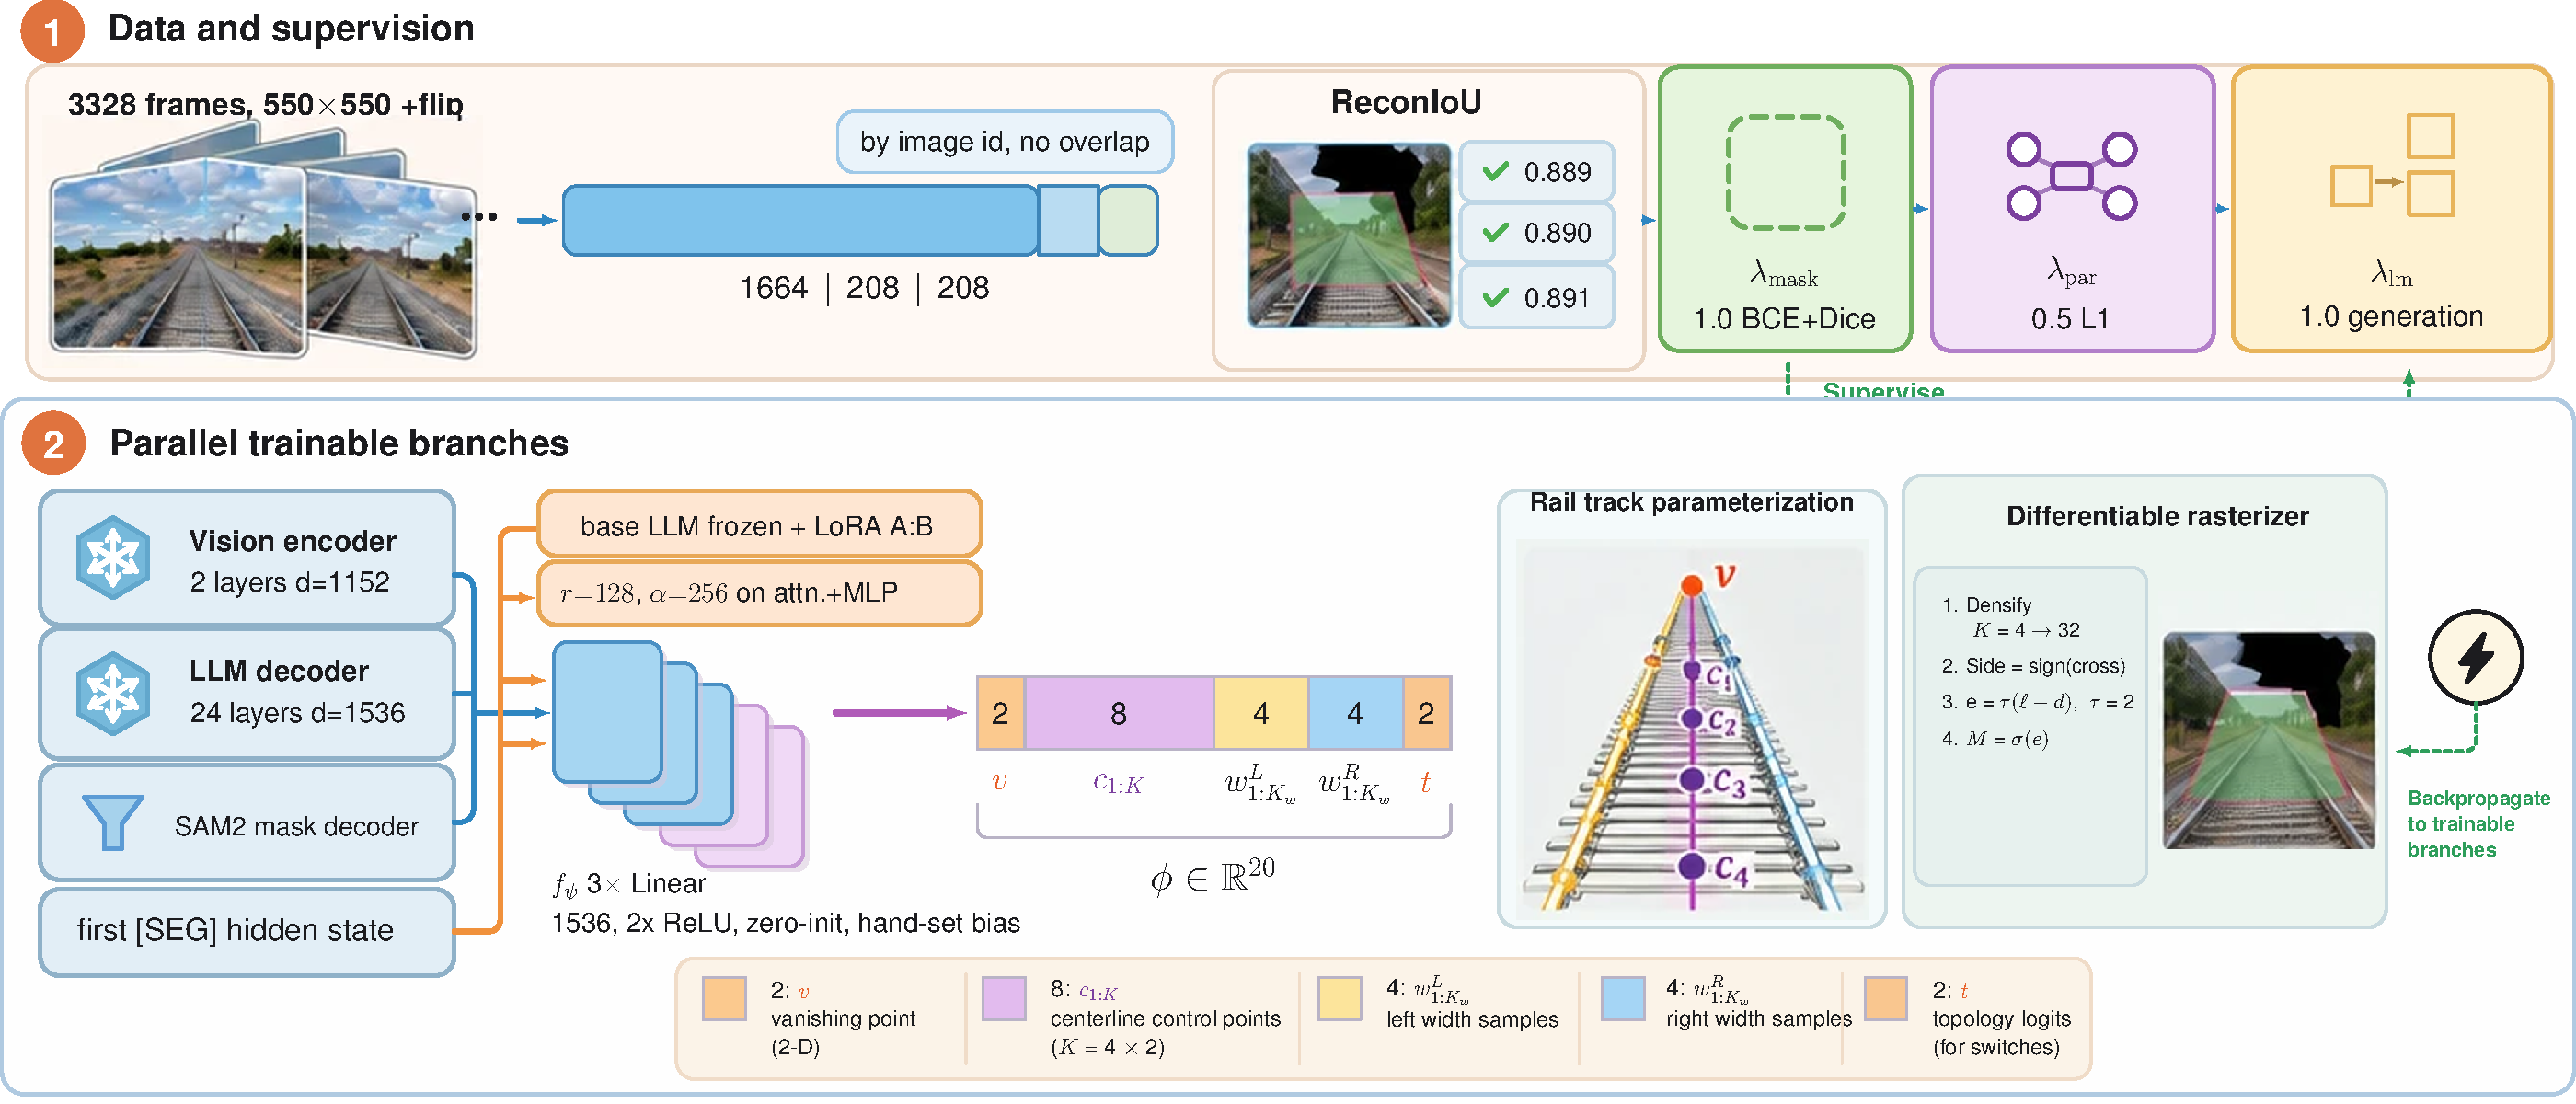
\includegraphics[width=\textwidth]{figures/ecf_pipeline_vec.pdf}%
\caption{Data, supervision, and the trainable branches. Band~1: the $3328$-frame corpus ($550{\times}550$, original$\cup$hflip) with the $1664|208|208$ split by image id, the per-split ReconIoU of the reconstructed labels ($0.889/0.890/0.891$), and the three primary loss weights of the recipe ($\lambda_{\mathrm{mask}}{=}1.0$ BCE${+}$Dice, $\lambda_{\mathrm{par}}{=}0.5$ L1, $\lambda_{\mathrm{lm}}{=}1.0$ generation). Band~2: the frozen trunk (vision encoder, LLM decoder, SAM2 mask decoder) carries LoRA ($r{=}128$, $\alpha{=}256$ on the LLM attention and MLP projections) and the ParamHead (three linear layers, zero-initialized, hand-set bias); the $20$ scalars of $\phih$ (legend: $2$ vanishing point, $8$ centerline, $4{+}4$ widths, $2$ topology) enter the differentiable rasterizer (densify $K{=}4$ to $32$, side sign, margin at $\tau{=}2$, $M{=}\sigma(e)$), and the dashed arrows mark the gradient that returns to the trainable branches.}
\label{fig:ecf_pipeline}
\end{figure*}

\subsection{Ego-Corridor Field}
\label{sec:phi}

The target in an ego-view rail frame is a perspective corridor, which we represent by a low-dimensional corridor field
\begin{equation}
\begin{aligned}
\phih
&= \big(
\mathbf{v},\;
\mathbf{c}_{1:K},\;
\mathbf{w}^{L}_{1:K_w},\;
\mathbf{w}^{R}_{1:K_w},\;
\mathbf{t}
\big) \\
&\in \mathbb{R}^{20},
\end{aligned}
\label{eq:phi}
\end{equation}
with $K{=}4$ centerline control points ($8$ coordinates), $K_w{=}4$ left/right width samples, a 2-D vanishing point $\mathbf{v}$, and $2$ topology logits $\mathbf{t}$ reserved for forks.
Centerline and vanishing-point coordinates live in image-normalized $[0,1]$, and widths are positive fractions of the image short side; a Rail-Path Verifier on $\mathbf{t}$ is \emph{not} trained, and we do not claim fork disambiguation.

The twenty scalars are budgeted by what the geometry has to bend. Four centerline points carry one inflection, which covers the straight, the gently curving and the strongly curving frames of the benchmark, and four width samples per side let the near field widen without forcing the far field to do the same. The remaining four slots are the anchor and the topology. The carrier compresses a $550{\times}550$ mask by about four orders of magnitude, and Section~\ref{sec:train} measures what survives.

Every coordinate is image-normalized, so the field does not depend on the resolution at which it is rendered, and every width is a fraction of the short side, so the same $\phih$ stays meaningful when the aspect ratio changes. The horizontal flip used in training is a closed-form involution on the parameters. The horizontal coordinate of each control point and of the vanishing point maps to one minus itself, the left and right width slots exchange roles, and the two topology logits exchange order. The flipped training copies are therefore exact.

A lightweight ParamHead $f_\psi$ maps $h$ to $\phih$: three linear layers with ReLU, last-layer weights zero-initialized, and a hand-set bias (vanishing point near $(0.5,0.2)$, centerline along the image axis, widths ${\approx}0.08$).
With zero initial weights it therefore starts as a plausible corridor rather than a random mask, as Figure~\ref{fig:ecf_forward} shows in detail: the \Seg{} hidden state through ParamHead to the corridor scalars and on to the per-slot curves the rasterizer consumes.
There is no output sigmoid or softplus: range constraints are applied inside the rasterizer (centerline clamped to $[0,1]$, widths $\ge 10^{-4}$).

The initialization is a prior rather than a random start. With the last layer at zero the head returns its bias at step zero, and that bias already describes a corridor running up the image axis. The first mask loss is therefore evaluated on a plausible corridor, and the gradient reaching $f_\psi$ corrects a shape instead of searching for one. The head is kept small on purpose, with $4.75$\,M parameters against a $2316.2$\,M frozen backbone, so the capacity for the task sits in the LoRA-adapted language model.

\subsection{Differentiable rasterization}
\label{sec:rast}

The differentiable rasterizer $\cR$ turns $\phih$ into a soft mask $M \in (0,1)^{H \times W}$: control points are scaled to pixels and densified along the polyline, and for each pixel a distance $d$ to the polyline is compared to a side-dependent width $\ell$ (mean left width if the signed offset is positive, mean right width otherwise):
\begin{equation}
\begin{aligned}
M &= \sigma\!\big(\tau\,(\ell - d)\big), \\
\hat{M} &= [M \ge 0.5],
\end{aligned}
\label{eq:rast}
\end{equation}
with temperature $\tau{=}2$; we call $e{=}\tau(\ell-d)$ the margin; Figure~\ref{fig:ecf_rast} expands the rasterizer one operation at a time.

Two operations sit between the scalars and the sigmoid. Densification joins the four control points into a polyline and resamples it to thirty-two points, so the distance field sees a curve rather than four vertices and the far field, where consecutive control points are far apart in pixels, does not develop polygonal corners. The distance $d$ of a pixel is then the minimum point-to-segment distance over the thirty-two segments, and the signed offset is measured along the left normal of the nearest segment. Only the sign of that offset is used, because the width on each side enters as a single scalar.

The margin is the only quantity the sigmoid sees, and it is what carries the gradient from the mask back to the parameters. The distance $d$ is Lipschitz in pixel position with constant one, the width $\ell$ is linear in the width slots, and $\sigma$ is smooth, so $\partial M/\partial \phih$ exists away from the centerline, where the side switches and the width jumps if the two sides differ, and away from the set where two segments are equidistant. Both sets are measure zero, and the jumps inside $\cR$ do not block the mask loss from reaching $f_\psi$. The temperature fixes the width of the soft band. At $\tau{=}2$ the ten to ninety percent transition spans about $2.2$ pixels at $550{\times}550$, narrow enough that the soft mask and the thresholded mask agree almost everywhere, and wide enough that a pixel just outside the boundary still receives a gradient.

The corridor $\cR$ renders is therefore a constant-width capsule around the polyline: the $K_w$ width samples enter only through their per-side mean, so a width profile \emph{along} the corridor is not currently modeled and the $\mathbf{w}^{L},\mathbf{w}^{R}$ slots act as a low-dimensional width control rather than as a dense envelope.
The vanishing point $\mathbf{v}$ is part of $\phih$ and is supervised in the parameter loss; occupancy itself is a distance-to-polyline field, not a ray-cast from $\mathbf{v}$.
Because $\sigma$ is smooth, mask losses back-propagate into $f_\psi$ and into the LoRA that produces $h$.
Figure~\ref{fig:framework} renders the evaluated forward path end to end, Figure~\ref{fig:ecf_forward} details the ParamHead mapping from $h$ to the corridor scalars, Figure~\ref{fig:ecf_pipeline} shows how the training signal is assembled and split across the trainable branches, and Figure~\ref{fig:ecf_rast} records where each step's gradient comes from.

\subsection{Training}
\label{sec:train}

Let $M^{gt}$ be the rasterized ground-truth rail mask and $\phih^{gt}$ a geometry-derived label (offline mask$\to$centerline/width/vanishing-point; train/val/test median ReconIoU $0.889/0.890/0.891$, supplementary material, Section~D).
Figure~\ref{fig:ecf_pipeline} lays out this recipe: the $3328$-frame corpus with its $1664|208|208$ split, the three loss weights, and the trainable branches that the gradient reaches.

The label is derived once, offline, from the annotation polygon. The polygon is rasterized, its medial axis gives an ordered centerline from the near field to the far field, and the width on each side is read by casting rays normal to the centerline until they leave the mask. The vanishing point comes from the two boundary lines of the corridor, and the topology logits come from the branch structure of the skeleton, which is trivial on single-rail frames. The procedure is deterministic and consumes only the released masks, so the parameter supervision adds no annotation cost.

The check on that label is reconstruction IoU. We render $\phih^{gt}$ with a non-learned reference renderer and compare the result to the original mask under the same IoU used for evaluation. The median is $0.889$ on train, $0.890$ on val and $0.891$ on test, so a twenty-dimensional corridor reproduces about nine tenths of the annotated region. The remaining tenth is the part of the annotation that the parameterization does not carry, so the figure bounds the label rather than the trained decoder.

The primary loss is
\begin{equation}
\begin{aligned}
\mathcal{L}
&= \lambda_{\mathrm{mask}}\mathcal{L}_{\mathrm{mask}}(\cR(\phih), M^{gt}) \\
&\quad + \lambda_{\mathrm{par}}\mathcal{L}_{\mathrm{param}}(\phih, \phih^{gt}) \\
&\quad + \lambda_{\mathrm{lm}}\mathcal{L}_{\mathrm{LM}},
\end{aligned}
\label{eq:loss}
\end{equation}
with $\lambda_{\mathrm{mask}}{=}1.0$, $\lambda_{\mathrm{par}}{=}0.5$, and $\lambda_{\mathrm{lm}}{=}1.0$ (generation); $\mathcal{L}_{\mathrm{param}}$ is an L1 on the non-topology coordinates, and $\mathcal{L}_{\mathrm{mask}}$ a sum of BCE and Dice on the soft raster, with SAM2 mask/dice losses replaced by a finite zero on this path (supplementary material, Section~F).

The reported training recipe also includes a weak width-monotonicity term ($0.1$), a far-row mask weight ($\gamma{=}1.0$), and small auxiliary weights on the topology logits and the frozen Verifier head (supplementary material); we do \emph{not} claim these as contributions---a later physics-heavy recipe failed to help far-field IoU and is not a main-table variant.

\textbf{Optimization.} LoRA ($r{=}128$, $\alpha{=}256$) on the LLM's attention and MLP projections, with the vision encoder frozen and ParamHead trainable, under AdamW at learning rate $4{\times}10^{-5}$ with mixed-precision fp16 and gradient clipping at $0.5$.
The reported checkpoint is a single $133{,}120$-iteration schedule on orig$\cup$hflip (3328 frames, 10 repeats, 4 epochs), initialized from the official InternVL3-2B Sa2VA weights (supplementary material, Section~F).

\textbf{Inference.} Generate the referring completion, take the first \Seg{} hidden state, $f_\psi \to \cR \to$ threshold $0.5$, all in \textbf{fp32}; fp16 evaluation is never used, since in our runs it collapses \Seg{} decoding.
The decode is one head application and one rasterization, with no mask prompt loop and no autoregressive repair, so a frame cannot depend on the mask predicted for another frame.
Figure~\ref{fig:framework} summarizes this evaluated forward path end to end.

% Fig.4 的浮动块放在 Training 小节之后，使它与 Fig.3 之间隔有实质正文，
% 避免两张全宽流程图在同一页背靠背堆叠（LaTeX 对相邻 figure*[t] 会连续堆到同一页顶）。
% Fig.5（rast）改用 [b]（页底，需 main.tex 的 dblfloatfix）：Fig.3 前移后它曾与
% Fig.6（dataset）同落一页且仅隔图注 → 改页底后可与之分居页顶/页底。
\begin{figure*}[b]
\centering
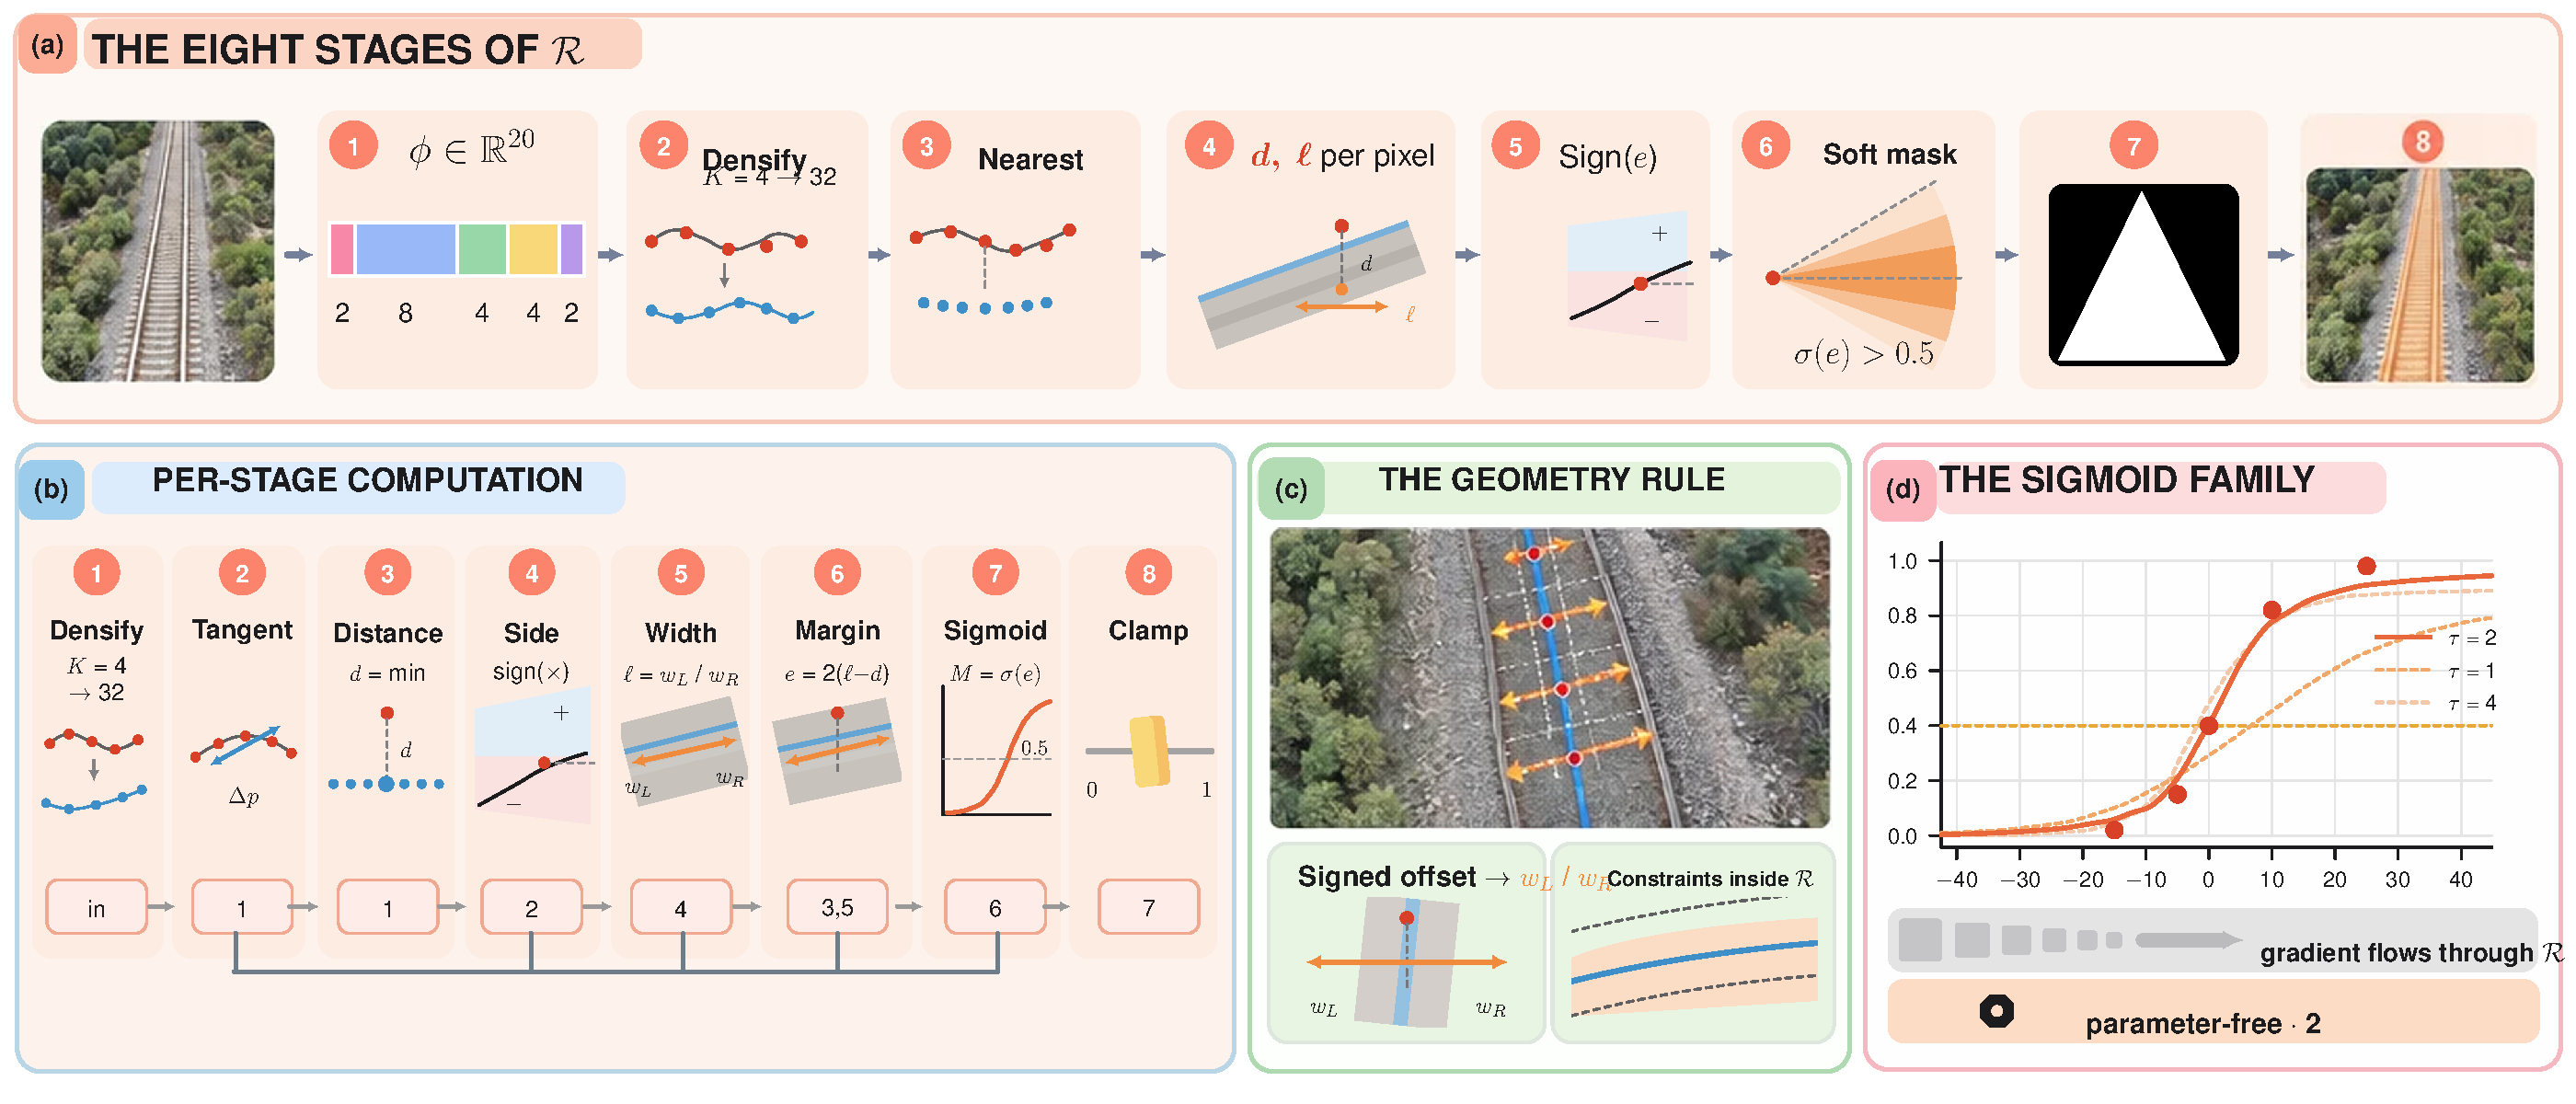
\includegraphics[width=\textwidth]{figures/ecf_rasterizer_vec.pdf}%
\caption{The differentiable rasterizer, operation by operation, on a test frame.
(a)~the eight stages that turn $\phih$ into the deployed mask, from the $20$ scalars through densification to the thresholded mask.
(b)~the same stages as explicit computations with their dependency badges: stage~$1$ is the only fan-out point and stage~$6$ the only two-input merge, so the chain stays strictly serial apart from the margin $e{=}\tau(\ell-d)$ at $\tau{=}2$.
(c)~the geometry rule on a test frame: the signed offset selects the left or right width, and the range constraints are applied inside $\cR$.
(d)~the $\sigma$ family for the temperatures the rasterizer admits; every member is smooth, so the mask loss crosses $\cR$ into $f_\psi$ and on into the LoRA, and the rasterizer itself holds no parameters.
The mask-production stage costs $2.90$\,ms of rasterization plus $2.30$\,ms of head evaluation, i.e.\ $2.42\%$ of the $214.6$\,ms end-to-end latency.}
\label{fig:ecf_rast}
\end{figure*}
